\documentclass[english,aspectratio=169]{beamer}
\usefonttheme{serif}
\usepackage[utf8]{inputenc}
\usepackage{pxfonts} % Or palatino or mathpazo
\usepackage{eulervm}
\usepackage{tabularx,booktabs}
\usepackage{longtable}
\newcolumntype{Y}{>{\centering\arraybackslash}X}
\usepackage{multirow}
\usefonttheme{serif}
\usepackage{xcolor}
\usepackage{soul}
\newcommand{\mathcolorbox}[2]{\colorbox{#1}{$\displaystyle #2$}}

% \usetheme{Madrid}}
\useinnertheme{rectangles}
\useoutertheme{infolines}

\definecolor{DarkPurple1}{RGB}{32,12,37}
\definecolor{Plum}{RGB}{184,13,72}
\definecolor{Rose}{RGB}{255,86,87}
\definecolor{Red}{RGB}{255,0,0}
\definecolor{DarkRed1}{RGB}{75,21,21}
\definecolor{DarkRed2}{RGB}{145,12,7}

\definecolor{Brown}{RGB}{110,54,42}

\definecolor{Orange1}{RGB}{242,151,36}
\definecolor{Orange2}{RGB}{244,129,83}
\definecolor{Mustard}{RGB}{253,179,56}
\definecolor{Gold}{RGB}{254,174,2}
\definecolor{LightYellow}{RGB}{241,226,160}
\definecolor{Tan}{RGB}{225,221,191}

\definecolor{Green}{RGB}{76,131,122}
\definecolor{Gray}{RGB}{242,242,242}
\definecolor{DarkGray1}{RGB}{127,127,127}
\definecolor{DarkGray2}{RGB}{64,64,64}

\definecolor{BlueGrey}{RGB}{99,143,169}
\definecolor{DarkBlue1}{RGB}{4,37,58}
\definecolor{DarkBlue2}{RGB}{2,81,150}
\definecolor{DarkTeal1}{RGB}{55,108,138}
\definecolor{DarkTeal2}{RGB}{43,106,108}
\definecolor{DarkTeal3}{RGB}{45,129,131}
\definecolor{Aqua}{RGB}{131,211,212}


\definecolor{links}{HTML}{2A1B81}

% \pagecolor{DarkTeal}

\setbeamercolor{title}{fg=DarkRed2}
\setbeamercolor{navigation symbols}{fg=Rose, bg=DarkRed2}
\setbeamercolor{frametitle}{fg=DarkRed1,bg=Mustard!30}
\setbeamercolor{section in head/foot}{fg=Brown,bg=Mustard!30}
\setbeamercolor{subsection in head/foot}{fg=Brown,bg=Mustard!10}
\setbeamercolor{author in head/foot}{fg=Brown,bg=Mustard!30}
\setbeamercolor{title in head/foot}{fg=Brown,bg=Mustard!30}
\setbeamercolor{date in head/foot}{fg=Brown,bg=Mustard!30}
\setbeamercolor{normal text}{bg=white,fg=black}
\setbeamercolor{section in sidebar}{fg=Brown}
\setbeamercolor{section in sidebar shaded}{fg=Mustard}
\setbeamercolor{section in toc}{fg=DarkRed2}
\setbeamercolor{subsection in toc}{fg=DarkRed2!90}
\setbeamercolor{subsubsection in toc}{fg=DarkRed2!80}
\setbeamertemplate{enumerate items}[default]
\setbeamercolor*{enumerate item}{bg=DarkRed2,fg=Mustard}
\setbeamercolor*{enumerate subitem}{bg=DarkRed2,fg=Mustard}
\setbeamercolor*{enumerate subsubitem}{bg=DarkRed2,fg=Mustard}
\setbeamercolor*{itemize subsubitem}{bg=DarkRed2,fg=Mustard}
% \setbeamercolor{background canvas}{fg=DarkRed,bg=DarkTeal!10}
\setbeamertemplate{itemize item}{\color{DarkRed2}$\blacksquare$}
\setbeamertemplate{itemize subitem}{\color{DarkRed2}$\blacktriangleright$}

\setbeamercolor{caption name}{fg=DarkRed2}
\defbeamertemplate{section in toc}{square unnumbered}{%
    \leavevmode\leftskip=1.75ex%
    \llap{\textcolor{DarkRed2}{\vrule width1.85ex height1.85ex depth0ex}}%
    \kern1.5ex\inserttocsection\par}
\defbeamertemplate{subsection in toc}{square1 unnumbered}{%
    \leavevmode\leftskip=3.75ex%
    \llap{\textcolor{DarkRed2!90}{\vrule width1.2ex height1.2ex depth0ex}}%
    \kern1.5ex\inserttocsubsection\par}
\defbeamertemplate{subsubsection in toc}{square2 unnumbered}{%
    \leavevmode\leftskip=5.75ex%
    \llap{\textcolor{DarkRed2!80}{\vrule width0.8ex height0.8ex depth0ex}}%
    \kern1.5ex\inserttocsubsection\par}
\setbeamertemplate{headline}{}
\setbeamertemplate{section in toc}[square unnumbered]
\setbeamertemplate{subsection in toc}[square1 unnumbered]
\setbeamertemplate{subsubsection in toc}[square2 unnumbered]

\hypersetup{colorlinks,linkcolor=,urlcolor=links}
\usepackage{graphicx,wrapfig,lipsum}
\usepackage{amsmath}
\usepackage{multirow}
\usepackage{changepage}
\usepackage{tikz}
\usepackage{algorithm2e}
\usepackage{algorithmic}
\usetikzlibrary{positioning}
\usetikzlibrary{decorations, decorations.text,backgrounds}

\DeclareMathOperator*{\argmax}{arg\,max}
\DeclareMathOperator*{\argmin}{arg\,min}
\newcommand{\norm}[1]{\left\lVert#1\right\rVert}

\title{Optimal Views for CT: Formulation}
\author{Soumendu Majee}
\date{}

\begin{document}

\begin{frame}[plain,noframenumbering]
    \titlepage
\end{frame}

\AtBeginSection[]
{
  \begin{frame}[plain,noframenumbering]
    \frametitle{Table of Contents}
    \tableofcontents[
        currentsection,
        sectionstyle=show/shaded,
        subsectionstyle=show/show/hide]
  \end{frame}
}

\begin{frame}{Motivation}
	\begin{itemize}
	    \setlength\itemsep{2em}
		\item Conventional CT scanning typically uses uniformly spaced view-angles
		
		\item Problem: Large information loss in sparse-view acquisition
		
		\item Solution: Optimize view-angles to reduce information loss for a class of objects
		
		
	\end{itemize}
\end{frame}

\begin{frame}{Domain of View-angle Optimization}
	\begin{itemize}
	    \setlength\itemsep{2em}
		\item Continuous: view-angles chosen in $[0, 2\pi]$
		\begin{itemize}
		    \item Need to choose angle values in $[0, 2\pi]$
	    \end{itemize}
		
		\item \textbf{Discrete}: view-angles chosen among dense set of angles: $\theta = \{\theta_1, \cdots, \theta_M \}$
		\begin{itemize}
		    \item Need to choose indices in $\{ 1, \cdots, M \}$
		
	    \end{itemize}
		
		
	\end{itemize}
\end{frame}

\begin{frame}{How to Measure Optimality?}
	\begin{itemize}
	    \setlength\itemsep{2em}
		\item Optimal view indices: $I^* = \argmin_{I \subset \{ 1, \cdots, M \}, |I|=P} c(I)  $
		
		\item Cost $c(I) = \text{rmse}(x^0, R(x^0,I))$ 
		\begin{itemize}
		    \item $x^0$ : Ground truth CT object for training
		    \item $R(x^0,I)$ : Image reconstructed with simulated data generated from $x^0$ using view indices in $I$
		    \item Other image quality measures can also be used
		
	    \end{itemize}
		
		
	\end{itemize}
\end{frame}

\begin{frame}{MBIR CT Reconstruction $R(x^0,I)$}
	\begin{itemize}
	    \setlength\itemsep{1em}
		\item Full set of view-angles: $\theta = [\theta_1, \cdots, \theta_M ]^\top$
		
		\item At angle $\theta_i$
		\begin{itemize}
		    \item Projection matrix: $A_{i}$
		    
		    \item Photon-counts: $\lambda_i \sim \text{Poisson}\left(\lambda^0 \exp (-A_{i}x^0) \right)$
		    
		    \item Transmission measurements: $ y_i = - \log\left(\frac{\lambda_i}{\lambda^0}\right) $
		
	    \end{itemize}
	    
		
		\item With subset of all view-angles: $I = \{i_1, i_2, \cdots, i_K \}$
		
		\begin{itemize}
		    \item Projection matrix: $A_I = [ A_{i_1}^\top, \cdots, A_{i_K}^\top ]^\top$
		    
		    \item Photon-counts: $\lambda_I = [ \lambda_{i_1}^\top, \cdots, \lambda_{i_K}^\top ]^\top$
		    
		    \item Transmission measurements: 	$y_I = [ y_{i_1}^\top, \cdots, y_{i_K}^\top ]^\top$
		
	    \end{itemize}
		
		\item $-\log p\left( y_I | x \right) \approx \frac{1}{2} \norm{y_I - A_I x}^2_D $, where $D=\text{diag}(\lambda_I)$
		
		\item $R(x^0,I) = \argmin_x \left\{ \frac{1}{2} \norm{y_I - A_I x}^2_D + h(x) \right\}$
		
		
	\end{itemize}
\end{frame}

\begin{frame}{Optimizing View-angles}
	\begin{itemize}
	    \setlength\itemsep{2em}
		\item Greedy approach
		
		\begin{algorithm}[H]
        \begin{algorithmic}[1]
        \STATE $I = \{\}$
        \WHILE{$|I|<P$}
            \STATE  $i = \argmin_{i \in \{1,\cdots,M \} } c(I \cup \{ i \})$
            \STATE $I = I \cup \{ i \}$
        \ENDWHILE
        
        \end{algorithmic}
        \label{alg:angle_greedy}
        \end{algorithm}
        
	\end{itemize}
	
\end{frame}


\begin{frame}{Toy Problem}
	\begin{itemize}
	    \setlength\itemsep{2em}
		\item Set up small toy problem where the optimal views can be computed via brute-force
		\begin{itemize}
		    \item Phantom: Downsampled shepp-logan phantom $16\times16$
		    \item Search for "best" $4$ view-angles among equi-spaced $16$ angles
		    \item Evaluate all ${16 \choose 4} = 1820$ possibilities
	    \end{itemize}
		
		
	    \item Used svmbir (\url{https://svmbir.readthedocs.io/en/latest/}) iterative reconstruction with MRF prior
	    
        
	\end{itemize}
	
\end{frame}


\begin{frame}{Toy Problem: Results}
	\begin{itemize}
	    \item Four equi-spaced angles: $0, 45, 90, 135$ degrees
	    \item Four optimal angles: $22.5, 78.75, 101.25, 135$ degrees
		\item Reconstruction with qui-spaced $4$ views: small features missing
        
	\end{itemize}
	
	\begin{figure}
    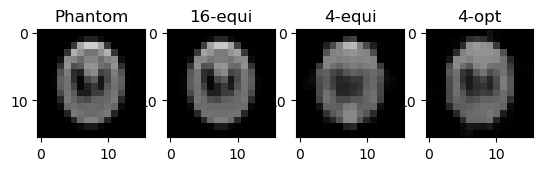
\includegraphics[scale=1.0]{Figs/plot_recon_compare.png}
    \end{figure}
	
\end{frame}

\bibliographystyle{IEEEtran}
\setbeamertemplate{bibliography item}{\insertbiblabel}
\bibliography{ref.bib}

\end{document}

